
\section{Appendix: Direct Calculation of $\sigma$}
\label{Sec:AppDirSig}

In our work, we used $\widehat{SE}$ to form an estimator for $\sigma$ when calculating the null distribution.  We developed another version of a differentially-private ANOVA that calculates $\sigma$ directly using a portion of the privacy budget.  We first define a generalized variance and prove the sensitivity bounds on this quantity.

\begin{definition}[$\var_q$] \label{def:varq} Given a database \x with $k$ groups and $n_j$ entries in the $j$-th group, the $\var_q$ calculation is defined as
\begin{equation*}
\var_q = \sum_{i=1}^N \lvert y_{i} - \overline{y} \rvert^q
\end{equation*}
where $q$ is a positive real number.
\end{definition}

\begin{theorem}[\varq-Sensitivity] \label{thm:varqSens} 
The sensitivity of \varq is bounded above by
$$ \frac{N-1}{N^q} + 1 $$
when $q<1$, and is bounded above by
$$ (N-1)(1-(1-1/N)^q) + 1 $$
when $q>1$. Note that these both give a bound of $2-1/N$ when $q=1$.
\end{theorem}

\begin{proof}
Consider databases \x and \xprime which differ in entry $r$. Recall that the sensitivity of the grand mean is $1/N$. Let $t_i = \left\vert  y_i - \grand \right\vert ^q$. When $q<1, t_i$ is a concave function with positive range, so the worst case sensitivity is between $ y_i - \grand = 0$ and $ y_i - \grand = 1/N$. That is, 
\begin{align*}
\Delta t_i &= \left\vert t_{i}(0) - t_i\left(\frac{1}{N}\right) \right\vert \\
	&= \left( \frac{1}{N} \right)^q.
\end{align*}
%
Every single term can be affected by at most $\left( \frac{1}{N} \right)^q$, except the term $r$, which can change by $1$. So, 
\begin{align*}
\Delta \varq &\le \left\vert (N-1)(\frac{1}{N})^q + 1 \right\vert \\
	&= \frac{N-1}{N^q} + 1.
\end{align*}
%
When $q>1, t_i$ is convex. The worst case sensitivity is between  $y_i - \grand = 1$ and $y_i - \grand = 1-1/N$ Then,
\begin{align*}
\Delta \varq \le \left\vert (N-1)(1-(1-\frac{1}{N})^q) + 1 \right\vert.
\end{align*}
\end{proof}

We again use the Laplace mechanism, and the sensitivity of a database's variance follows directly from Thm.~\ref{thm:varqSens}:

%In our work, the calculation of $p$-values did not take up any portion of the privacy budget, since we were able to use the \mse as an estimate of the standard deviation when we calculated the null distribution. However, if this hadn't been the case, we would have had to allocate a portion of the privacy budget to this calculation, and sacrifice some of the accuracy of our test statistic. One might ask how much this would affect the statistic's power. 

%To answer this question, we run the same power analysis as described in previous sections, but allocate part of the privacy budget to a differentially-private calculation of the variance of the data. We use the Laplace mechanism for our differentially private mechanism, so need to determine its sensitivity, which is stated below and follows directly from Thm.~\ref{thm:varqSens}.

\begin{corollary}
\label{thm:varsens}
The sensitivity of the variance of a database is bounded above by
$$ 3 + 1/N^2 - 3/N.$$
\end{corollary}

Algorithm~\ref{alg:F1hatVar} divides the privacy budget into $\rho_1$ for the \sa, $\rho_2$ for the \se, and $\rho_3$ for the $\var$ calculations respectively.  The values of $\rho$ are provided as input along with the database \x and the $\eps$ value. When $\widehat{SE}$ is used as the $\sigma$ estimate, we found a 70-30 split of the privacy budget between \sa and \se was optimal (Figure~\ref{Fig:f1-epsfrac}).   In the power analysis of Algorithm~\ref{alg:F1hatVar}, we vary the proportion of the privacy budget dedicated to the \var calculation.  We fixed the proportion of the privacy budget for $\rho_1$ and $\rho_2$ to be a 70-30 split budget not used by $\rho_3$ (the \var calcuation).  


%The resulting differentially-private algorithm is identical to our previous algorithms, except part of the privacy budget is allocated to a variance calculation, which is outputted in addition to the other calculations. The algorithm, which follows, additionally takes as input parameters $\rho_1, \rho_2,$ and $\rho_3$, where each $\rho$ is the fractional amount of the privacy parameter to budget to the $\sa, \se$ and $\var$ calculations respectively.

\begin{algorithm}
    \begin{algorithmic}
        \STATE \textbf{Input:} Database \x, $\eps$ value, $\rho_1, \rho_2, \rho_3$
        \STATE Compute $\widehat{\sa} = \sa + Z_1$ where $Z_1\sim \lap\left(\frac{4}{\eps \rho_1}\right)$
        \STATE Compute $\widehat{\se} = \se+ Z_2$ where $Z_2\sim \lap\left(\frac{3}{\eps \rho_2}\right)$
        \STATE Compute $\!\!\widehat{\var} \!\!= \!\!\var \!\!+\! Z_3\!$ where  $\!Z_3 \!\sim\! \lap\!\!\left(\! \frac{3\!+\!1/N^2\! - \!3/N}{\eps\rho_3} \!\right)$
        \STATE Compute $\widehat{F_1} = \frac{\widehat{\sa}/(\k-1)}{\widehat{\se}/(\dbsize-\k)}$
        \STATE \textbf{Output:} $\widehat{F_1}, \widehat{\sa}, \widehat{\se}, \widehat{\var}$
    \end{algorithmic}
    \caption{Differentially private $F_1$-statistic with direct calculation of variance}
     \label{alg:F1hatVar}
\end{algorithm}

Unsurprisingly, allocating part of the budget to calculating the standard deviation negatively impacts the statistical power of the test (Fig.~\ref{Fig:multiple-rhos}). However, it is surprising that this allocation does not impact the power of the test more strongly, since \var has a larger sensitivity and requires adding noise to smaller values than the \sa and \se. 

%Power analysis proceeds as in previous work, although we additionally experimentally optimize $\rho_1, \rho_2,$ and $\rho_3$. In our analysis, the choice of $\rho_1$ and $\rho_2$ is always a 70-30 split of the privacy budget not used by $\rho_3$; this choice was made due to the fact that when the standard deviation is estimated, a 70-30 split of the privacy budget between the \sa and \se turns out to be optimal. Unsurprisingly, as shown in Fig.~\ref{Fig:multiple-rhos}, allocating part of the budget to calculating the standard deviation negatively impacts the statistical power of the test. It is however surprising that it does not impact the power any more, since $\var$ has a larger sensitivity and requires adding noise to smaller values than the \sa and \se, since the residuals in the expression are squared.

\begin{figure}[h]
\centering
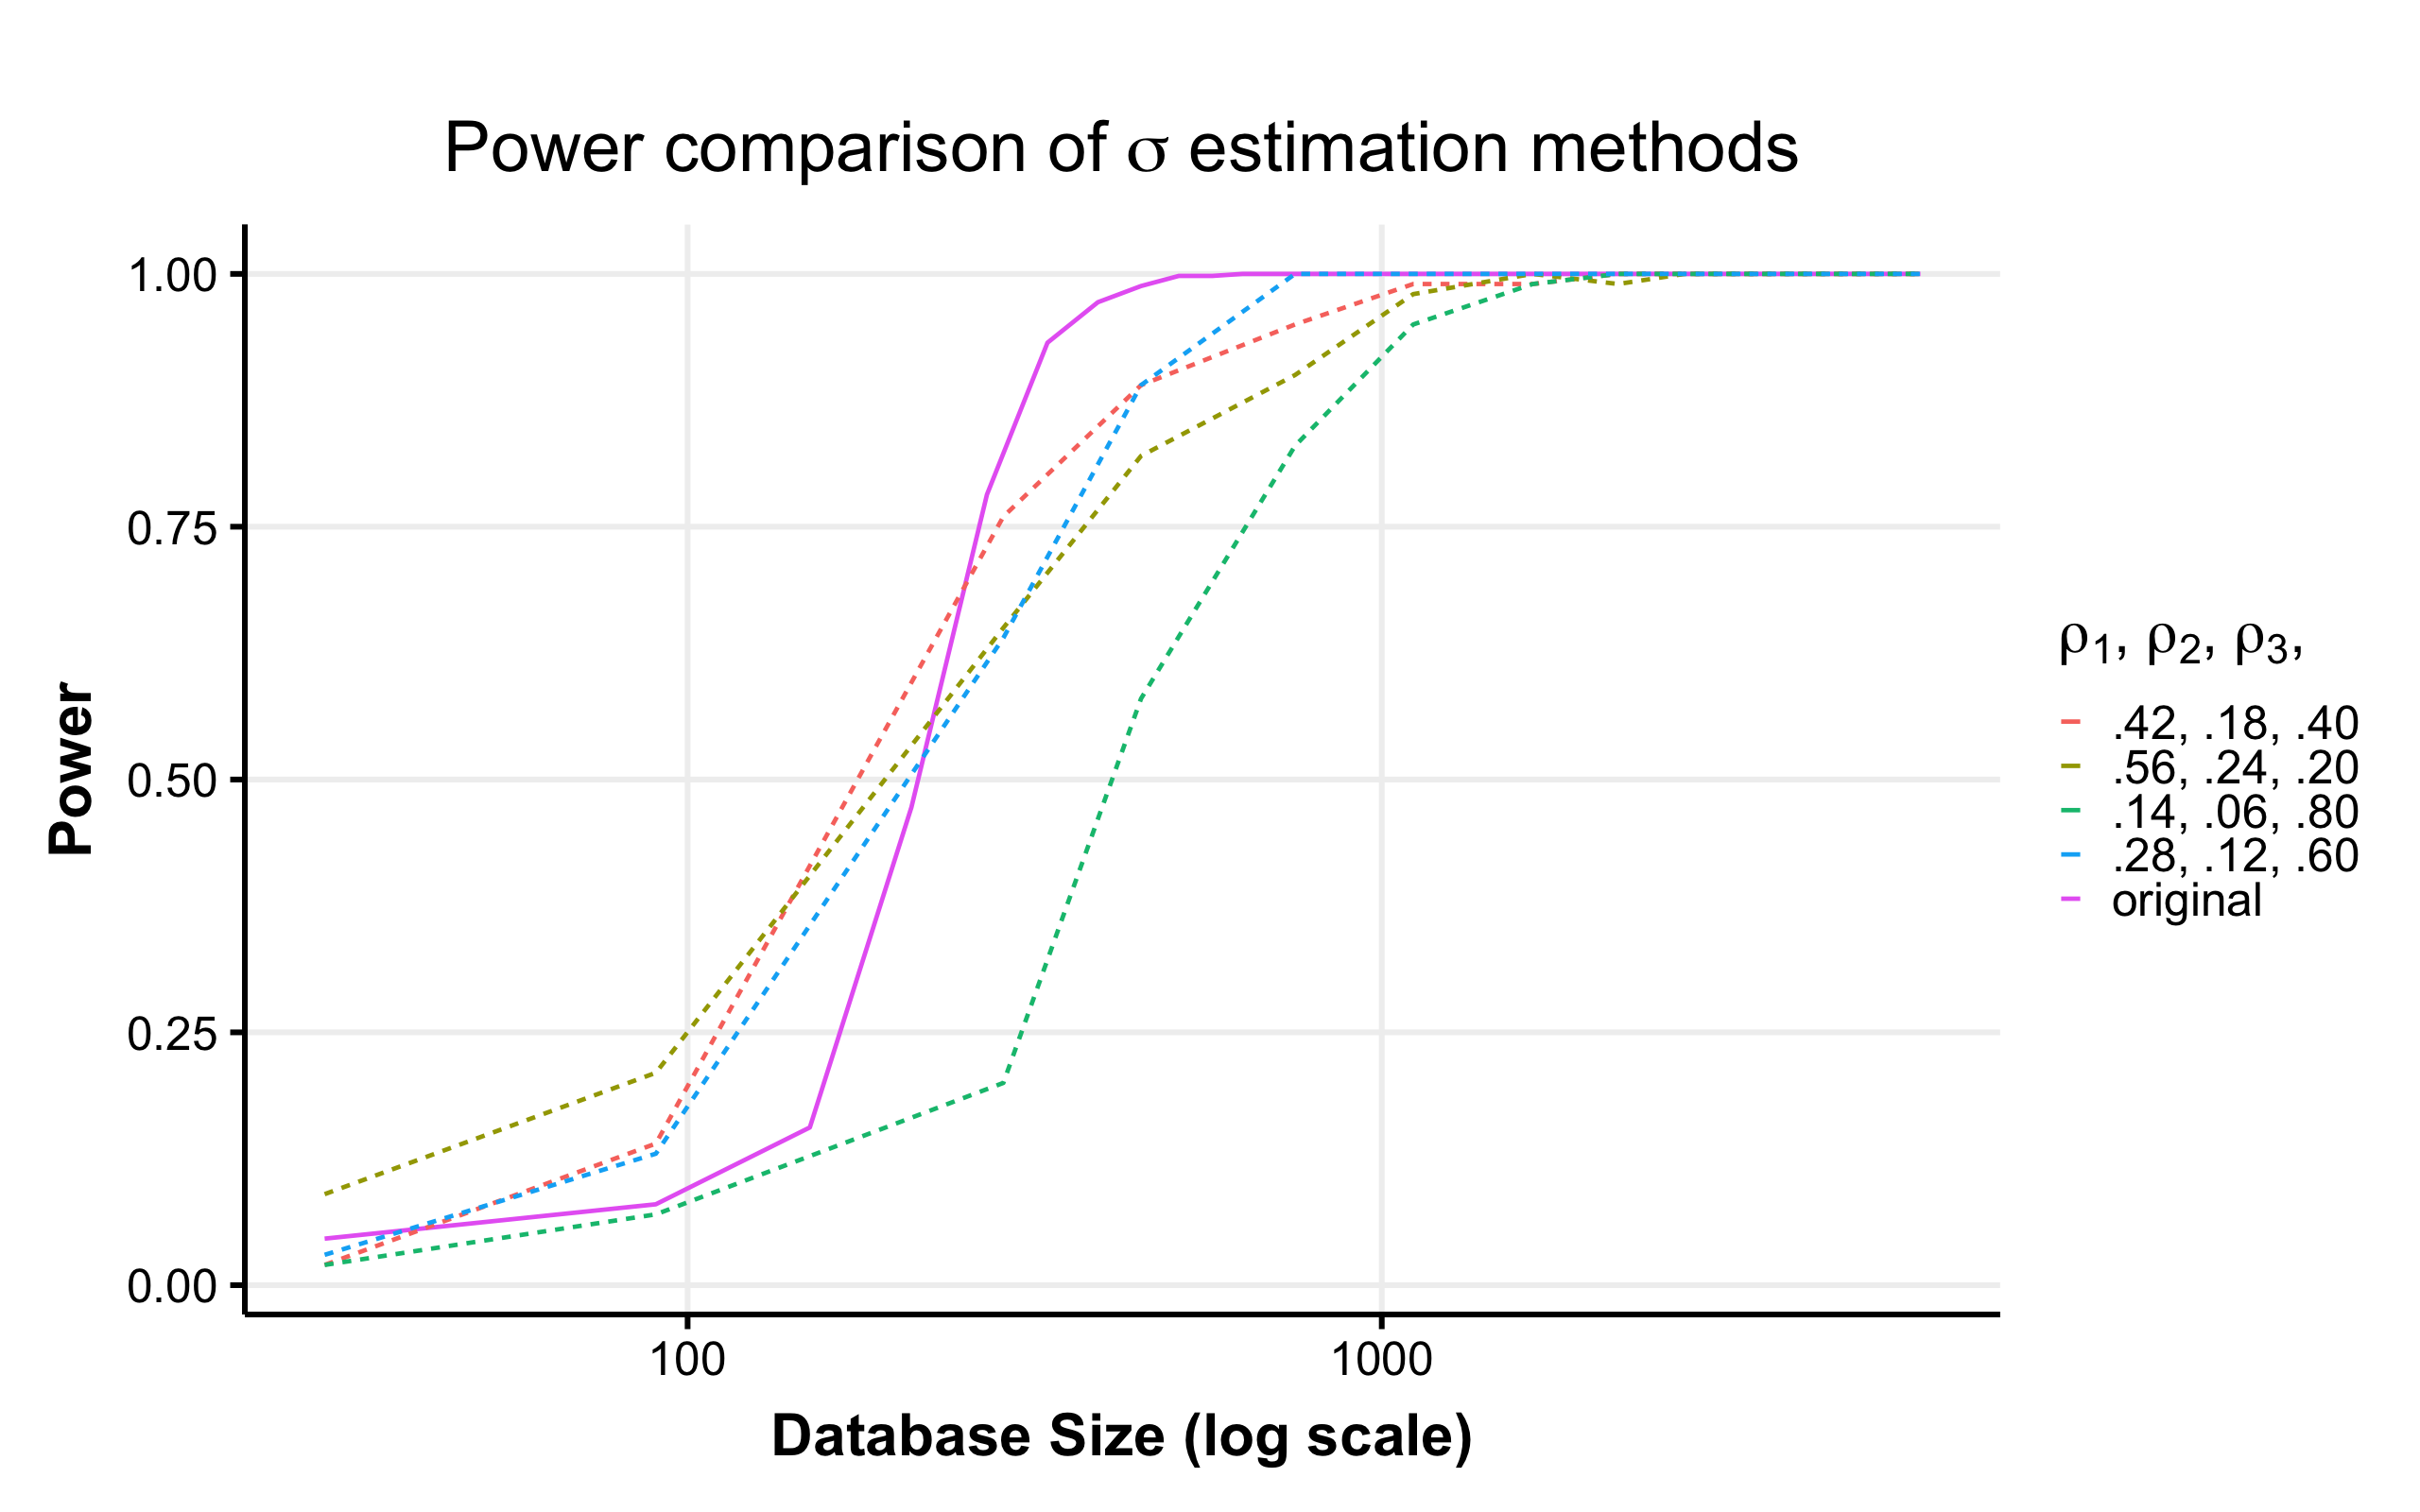
\includegraphics[width=\linewidth]{multiple-rhos.png}
\caption{The power of $F_1$ for a fixed $\epsilon$ value budgeted across \sa, \se, and \var calculations, with the portion of $\epsilon$ not allocated to $\rho_3$ allocated between $\rho_1$ and $\rho_2$ with a 70-30 split.\label{Fig:multiple-rhos}}
\end{figure}
